% The cycle structure of Frob_𝔓 = g acting on the n = 7 left cosets
% of H: one 3-cycle and one 4-cycle, so the pattern is 7 = 3 + 4.
% Source: book/tex/alg-NT/frobenius.tex (§ Frobenius elements control
% factorization) — asy.
\documentclass[border=2mm]{standalone}
\usepackage{tikz}
\usetikzlibrary{arrows.meta}
\usepackage{amssymb}
\usepackage{amsmath}
\begin{document}
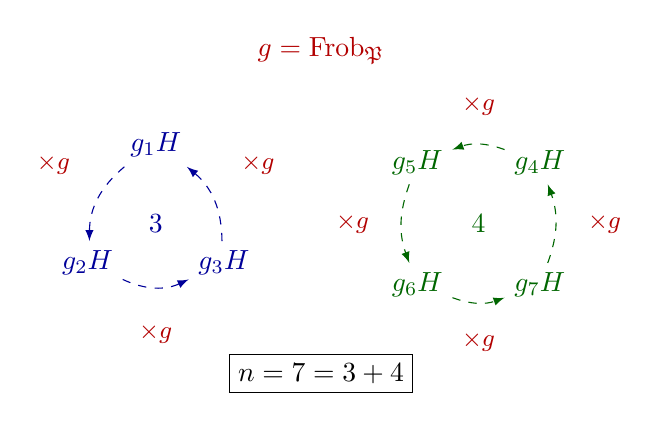
\begin{tikzpicture}[>=latex,
  lbl/.style={red!70!black},
  cos/.style={blue!60!black}]
  \node[lbl] at (0.2,2.2) {$g = \operatorname{Frob}_{\mathfrak{P}}$};
  % 3-cycle.
  \begin{scope}[shift={(-1.9,0)}]
    \node[cos] (A) at (90:1)  {$g_1H$};
    \node[cos] (B) at (210:1) {$g_2H$};
    \node[cos] (C) at (330:1) {$g_3H$};
    \draw[dashed, ->, cos] (A) to[bend right=25] (B);
    \draw[dashed, ->, cos] (B) to[bend right=25] (C);
    \draw[dashed, ->, cos] (C) to[bend right=25] (A);
    \node[lbl] at (150:1.5) {\small $\times g$};
    \node[lbl] at (270:1.4) {\small $\times g$};
    \node[lbl] at (30:1.5)  {\small $\times g$};
    \node[cos] at (0,0) {$3$};
  \end{scope}
  % 4-cycle.
  \begin{scope}[shift={(2.2,0)}]
    \node[green!40!black] (W) at (45:1.1)  {$g_4H$};
    \node[green!40!black] (X) at (135:1.1) {$g_5H$};
    \node[green!40!black] (Y) at (225:1.1) {$g_6H$};
    \node[green!40!black] (Z) at (315:1.1) {$g_7H$};
    \draw[dashed, ->, green!40!black] (W) to[bend right=20] (X);
    \draw[dashed, ->, green!40!black] (X) to[bend right=20] (Y);
    \draw[dashed, ->, green!40!black] (Y) to[bend right=20] (Z);
    \draw[dashed, ->, green!40!black] (Z) to[bend right=20] (W);
    \node[lbl] at (90:1.5)  {\small $\times g$};
    \node[lbl] at (180:1.6) {\small $\times g$};
    \node[lbl] at (270:1.5) {\small $\times g$};
    \node[lbl] at (0:1.6)   {\small $\times g$};
    \node[green!40!black] at (0,0) {$4$};
  \end{scope}
  \node at (0.2,-1.9) {$\boxed{n = 7 = 3+4}$};
\end{tikzpicture}
\end{document}
